\section{ХОД РАБОТЫ}

\subsection{Текст задания}

Разработанная программа должна производить нумерацию строк файла-источника
и сохранять пронумерованную версию файла-источника в указанный файл-приемник.

Разработанная программа должна быть написана с использованием условных выражений
и циклов, иметь возможность вывода справки по требованию пользователя.

\subsection{Детали реализации программы}

Выполнение разработанной программы можно логически разделить на следующие операции:

\begin{enumerate}
  \item разбор аргументов командной строки;
  \item чтение содержимого указанного файла;
  \item обработка данных (нумерация строк);
  \item запись результатов в указанный файл.
\end{enumerate}

Процесс работы программы приведен на рисунке~\ref{fig:process}.

\begin{figure}[htbp]
  \centering
  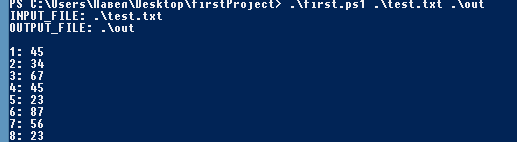
\includegraphics[width=150mm,height=40mm]{img/process}
  \caption{Процесс работы разработанной программы}\label{fig:process}
\end{figure}

\newpage

Содержимое исходного файла с данными \textit{test.txt} представлено на рисунке~\ref{lst:data}.
\begin{lstlisting}[caption=Содержимое исходного файла \textit{test.txt},label=lst:data]
  45
  34
  67
  45
  23
  87
  56
  23
\end{lstlisting}

В случае ошибочного ввода аргументов пользователь получит сообщение об ошибке,
представленное на рисунке~\ref{fig:error}.

\begin{figure}[htbp]
  \centering
  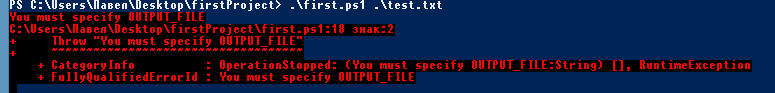
\includegraphics[width=150mm,height=20mm]{img/error}
  \caption{Вывод сообщения об ошибке при недостатке аргументов}\label{fig:error}
\end{figure}

Исходный текст разработанной программы расположен в приложении~А.

\newpage
